\documentclass{article}

\PassOptionsToPackage{numbers,sort&compress}{natbib}
\usepackage[preprint]{Styles/neurips_2025}
\usepackage[utf8]{inputenc}
\usepackage[T1]{fontenc}
\usepackage{amsmath}
\usepackage{amssymb}
\usepackage{array}
\usepackage{booktabs}
\usepackage{graphicx}
\usepackage{microtype}
\usepackage{placeins}
\usepackage{xcolor}
\usepackage{url}
\usepackage{hyperref}
\usepackage{tikz}
\usepackage{pgfplots}

\hypersetup{hidelinks}

\usetikzlibrary{arrows.meta,positioning,fit,calc,shapes.geometric}
\pgfplotsset{compat=1.17}

\makeatletter
\renewcommand{\@noticestring}{CSC6133 Deep Learning for Computer Vision Final Project Report}
\makeatother

\definecolor{ragblue}{HTML}{2F5597}
\definecolor{raggreen}{HTML}{3A7D44}
\definecolor{ragorange}{HTML}{C55A11}
\definecolor{ragred}{HTML}{A23B3B}
\definecolor{raggray}{HTML}{666666}
\urlstyle{tt}

\newcommand{\method}{Latent Conditioned Relation Scoring}
\newcommand{\acc}{Acc@1}
\newcommand{\acctopfive}{Acc@5}
\newcommand{\cf}{\mathrm{CF}}
\newcommand{\ce}{\mathrm{CE}}
\newcommand{\pp}{\,\mathrm{pp}}
\newcolumntype{L}[1]{>{\raggedright\arraybackslash}p{#1}}

\title{Latent Conditioned Relation Scoring for 3D Visual Grounding}

\author{%
  Che CHENG\\
  Student ID: 225015050\\
  CSC6133 Deep Learning for Computer Vision\\
}

\begin{document}

\maketitle

\begin{abstract}
This report summarizes the current state of a course project on relation-aware 3D visual grounding. The task is to identify a target object in a 3D scene from a natural-language expression, where many difficult examples require spatial relations such as ``near'', ``left of'', ``on'', or ``between''. The repository now contains a verified scene-disjoint Nr3D/ReferIt3D-style evaluation pipeline, a reproduced ReferIt3DNet baseline, hard-subset and coverage diagnostics, dense relation reranking experiments, and conditioned relation-scoring variants. The most reliable evidence is diagnostic: the reproduced baseline obtains 30.83\% \acc{} on 4,255 scene-disjoint test samples, while same-class clutter, high clutter, and multi-anchor subsets drop to 21.96\%, 16.07\%, and 11.90\%. Coverage analysis further shows that sparse top-5 anchor selection misses every annotated anchor in 33.95\% of baseline-wrong, anchor-evaluable cases. Method evidence is more qualified. A controlled three-seed Phase 4 rerun shows a conditioned relation architecture improves from 28.61\% to 30.50\% \acc{}, and removing viewpoint supervision gives a statistically similar 30.45\%. A near parameter-matched control remains much lower at 28.87\%, but random and shuffled viewpoint controls indicate that the gain should be framed as conditional architecture rather than explicit viewpoint learning. Counterfactual and latent-mode experiments are implemented and pass pilot validation, but full training remains future work.
\end{abstract}

\section{Introduction}

3D visual grounding maps a referring expression to one object in a reconstructed 3D scene. A system that receives ``the chair next to the desk'' must recognize candidate chairs, identify plausible desk anchors, and reason about the spatial relation between them. The task is therefore more structured than ordinary object classification: many examples are only resolvable through relation evidence, same-class distractor handling, and a speaker-dependent interpretation of spatial language.

This project studies that relational part of 3D grounding. The initial goal was to build a relation-aware grounding model that improves over a reproduced ReferIt3DNet-style listener. The repository has since evolved into a broader empirical study with scene-disjoint split recovery, frozen-logit baseline evaluation, hard-subset diagnostics, coverage analysis, dense reranking experiments, viewpoint-conditioned ablations, counterfactual training pilots, and latent relation-mode pilots. This report follows the current evidence rather than the original hypothesis: the best-supported contribution is \method{}, not explicit viewpoint supervision or completed anchor-chain reasoning.

This project contributes three course-level artifacts: a verified scene-disjoint evaluation pipeline, a diagnostic suite for hard-subset and anchor-coverage failures, and a controlled conditioned relation-scoring study. It is therefore framed as a reproducible empirical study with a conservative method signal, rather than as a state-of-the-art 3D grounding system.

\begin{figure}[!htbp]
  \centering
  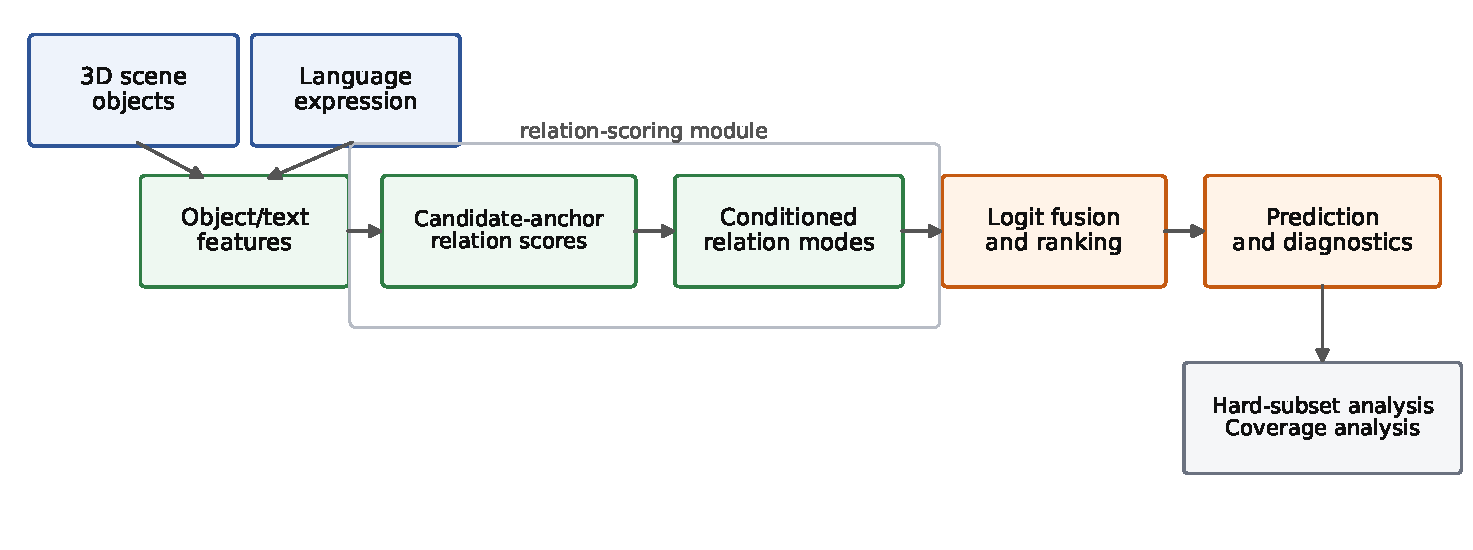
\includegraphics[width=\linewidth]{../../assets/figures/figure1_pipeline.pdf}
  \caption{Current project pipeline. The system keeps the object-centric grounding setup, adds relation-aware scoring over candidate-anchor pairs, and reports both predictions and diagnostics. The strongest method evidence supports a conditioned relation architecture, while the broader project contribution includes scene-disjoint evaluation and failure analysis.}
  \label{fig:pipeline}
\end{figure}

The project has three current-evidence conclusions. First, scene-disjoint grounding failures are concentrated in measurable hard subsets, especially same-class clutter and multi-anchor references. Second, sparse geometric anchor selection creates a real coverage bottleneck: dense all-pair candidate-anchor scoring can include anchor evidence that sparse top-$k$ selection misses. Third, the controlled method evidence supports conditional relation computation, but it does not support the claim that explicit viewpoint supervision is the source of the gain.

This distinction matters for a research-oriented course project. A less careful report could claim that viewpoint labels solve relational grounding. The current results do not justify that. Instead, the repository shows a more realistic research process: reproduce a baseline, identify where it fails, test relation mechanisms, preserve negative findings, and reframe the method claim when ablations contradict the initial explanation.

\paragraph{Code availability.}
Code and reproducibility artifacts are available at:\\
\url{https://github.com/checheng117/relation-aware-3d-grounding}.

\section{Related Work}

\paragraph{Datasets and task definitions.}
This project builds on ScanNet, a richly annotated RGB-D reconstruction dataset for indoor 3D scene understanding~\citep{dai2017scannet}. ReferIt3D introduced natural referring expressions for fine-grained 3D object identification, including the Nr3D/Sr3D settings used by many later grounding works~\citep{achlioptas2020referit3d}. ScanRefer studies the related problem of localizing language-described objects in ScanNet scenes~\citep{chen2020scanrefer}. These benchmarks make 3D grounding harder than category recognition because the target is often one among several same-class objects and the language may require relation, viewpoint, or anchor evidence.

\paragraph{3D visual grounding.}
Modern 3D grounding methods improve both proposal quality and cross-modal feature interaction. SAT adds 2D semantic assistance to the 3D listener~\citep{yang2021sat}. 3D-SPS avoids a strict detect-then-match pipeline by progressively selecting referred points with language guidance~\citep{luo2022sps}. BUTD-DETR decodes grounded objects from bottom-up objectness and top-down language cues rather than only selecting from fixed proposals~\citep{jain2022butd}. These systems are stronger and broader than the lightweight object-centric pipeline studied here; this report does not claim direct leaderboard comparison against them.

\paragraph{Relation reasoning and anchors.}
Natural referring expressions often name both a target and one or more anchors. InstanceRefer combines instance attributes, instance-to-instance relations, and global localization cues after reducing the candidate set~\citep{yuan2021instancerefer}. 3DVG-Transformer explicitly models proposal relations for relation-enhanced proposal generation and cross-modal disambiguation~\citep{zhao2021_3DVG_Transformer}. EDA decouples text into semantic components and densely aligns language with visual features~\citep{wu2023eda}. These works make clear that relation modeling and dense alignment are established ideas. The current project is narrower: it diagnoses coverage and hard-subset failures, then tests a controlled relation-scoring module. The repository includes anchor-chain parsing utilities, but Phase 4.5 diagnostics show that the conditioned scorer does not yet improve multi-anchor accuracy. For that reason, anchor-chain reasoning is treated as future work rather than a completed contribution.

\paragraph{Conditional computation.}
The method direction is related to mixture-of-experts and conditional computation, where a gate selects or weights different expert functions~\citep{jacobs1991adaptive,shazeer2017outrageously,fedus2022switch}. Here, the experts are pairwise relation scorers rather than generic feed-forward layers. The gate is conditioned on language features, which lets the relation module represent multiple relation modes without requiring explicit viewpoint labels.

\paragraph{Hard negatives and counterfactual training.}
Hard-negative objectives are widely used in visual-semantic retrieval and representation learning~\citep{faghri2018vse}. Counterfactually augmented data can also test whether a model learns the difference that matters for a decision~\citep{kaushik2020learning}. This project implements counterfactual relation learning as an auxiliary pilot objective. The current evidence is promising but small, so it is not used as the main claim.

\section{Method}

\subsection{Problem Setup}

Each sample contains a scene, a referring expression, a set of candidate objects, and a target object index. In the embedding-based training path, object embeddings have dimension 320 and language features have dimension 256. Let $o_i$ be the embedding of candidate object $i$, let $x$ be the utterance feature, and let $b_i$ be a base grounding logit. The relation module computes an additional score $r_i$, and the final logit is
\begin{equation}
  \ell_i = b_i + \lambda r_i .
  \label{eq:fusion}
\end{equation}
The training objective is cross-entropy over candidates unless an auxiliary loss is enabled.

\subsection{Pairwise Relation Scoring}

The basic relation module scores candidate-anchor pairs. For candidate $i$ and possible anchor $j$, a pair feature is formed from candidate, anchor, and language embeddings:
\begin{equation}
  h_{ij} = [o_i; o_j; x].
\end{equation}
A relation MLP produces a pair score $s_{ij}$. Candidate-level relation evidence is aggregated over anchors with a softmax temperature $\tau$:
\begin{equation}
  \alpha_{ij} = \mathrm{softmax}_{j}(s_{ij}/\tau),
  \qquad
  r_i = \sum_j \alpha_{ij}s_{ij}.
  \label{eq:anchor-aggregation}
\end{equation}
This design exposes a key practical issue: if useful anchors are not included in the anchor pool, no downstream scorer can recover the correct relational evidence. That is why the project includes explicit coverage diagnostics.

\subsection{Latent Conditioned Relation Scoring}

The current primary method generalizes the pairwise scorer into a language-conditioned mixture:
\begin{equation}
  s(i,j\mid x) = \sum_{k=1}^{K}\pi_k(x) f_k(o_i,o_j,x),
  \label{eq:latent-score}
\end{equation}
where $f_k$ is the $k$-th relation expert and $\pi_k(x)$ is a language-conditioned gate:
\begin{equation}
  \pi(x)=\mathrm{softmax}(W_g\,\mathrm{GELU}(U_gx+b_g)+c_g).
\end{equation}
When $K=1$, the model is a single relation expert. When $K>1$, the module can represent multiple latent relation modes. Earlier Phase 4 code used viewpoint-conditioned scoring, but the current interpretation is broader: viewpoint is one possible conditioning signal, not the validated source of improvement.

\subsection{Optional Counterfactual Loss}

The counterfactual objective is implemented as an auxiliary margin loss. Given target logit $\ell_y$ and a set of counterfactual negative logits $\ell_c$, the loss is
\begin{equation}
  \mathcal{L}_{\cf} =
  \frac{1}{|\mathcal{C}|}
  \sum_{c\in\mathcal{C}}\max(0, m+\ell_c-\ell_y).
\end{equation}
The total loss is
\begin{equation}
  \mathcal{L} = \mathcal{L}_{\ce} + \lambda_{\cf}\mathcal{L}_{\cf}.
\end{equation}
The pilot configuration uses margin $m=0.2$ and $\lambda_{\cf}=0.3$. Because the current pre-extracted embeddings store class IDs and feature vectors but not full 3D object metadata, the intended random hard-negative control cannot yet be activated reliably.

\section{Experimental Setup}

\paragraph{Data and splits.}
The trusted evaluation setting is the recovered scene-disjoint Nr3D/ReferIt3D-style split. The recovered dataset contains 41,503 samples over 641 scenes, and the main test split contains 4,255 samples. The split recovery is treated as a core artifact because scene overlap can overstate generalization in 3D grounding.

\paragraph{Metrics.}
The primary metrics are \acc{} and \acctopfive{}. \acc{} measures whether the top-ranked object is the ground-truth target, and \acctopfive{} measures whether the target is in the top five. Diagnostic tables also report subset counts, subset proportions, and percentage-point gaps relative to overall accuracy.

\paragraph{Evidence levels.}
The report distinguishes four evidence levels. Final evidence includes the scene-disjoint split recovery, baseline reproduction, hard-subset diagnostics, and coverage diagnostics. Controlled evidence includes Phase 4 architecture ablations and dense reranking comparisons. Pilot evidence includes one-epoch counterfactual and latent-mode runs. Pending evidence includes full 80-epoch latent-mode training, stronger random hard-negative controls, and multi-seed validation for pilot components.

\paragraph{Protocol boundary.}
The repository contains results from several protocols: frozen baseline logits, trained Phase 4 relation modules, and embedding-based Phase 5/6 pilots. These values should not be collapsed into a single leaderboard. The results section keeps them separated and labels protocol differences explicitly.

\paragraph{Reproducibility artifacts.}
The main split, evidence, and claim-boundary notes are documented under \path{course-line/}. Baseline, hard-subset, and coverage summaries are under \path{reports/}, including the coverage-diagnostics subdirectory. The controlled Phase 4 rerun uses seeds 42, 123, and 2026; its sanitized R001, R002, and R004 aggregate JSON records are under \path{reports/phase4_aggregates/}. These artifacts keep frozen-logit diagnostics, trained Phase 4 ablations, and Phase 5/6 pilots separated rather than merged into a single leaderboard.

\section{Results and Analysis}

\subsection{Baseline Failure Patterns}

The reproduced ReferIt3DNet baseline achieves 30.83\% \acc{} and 91.87\% \acctopfive{} on the scene-disjoint test split. The hard-subset diagnostics show that this average hides large failure concentrations. The subset script reports a slightly different computed overall value, 31.05\%, so Table~\ref{tab:hard-subsets} uses that diagnostic reference when computing gaps.

\begin{figure}[!htbp]
  \centering
  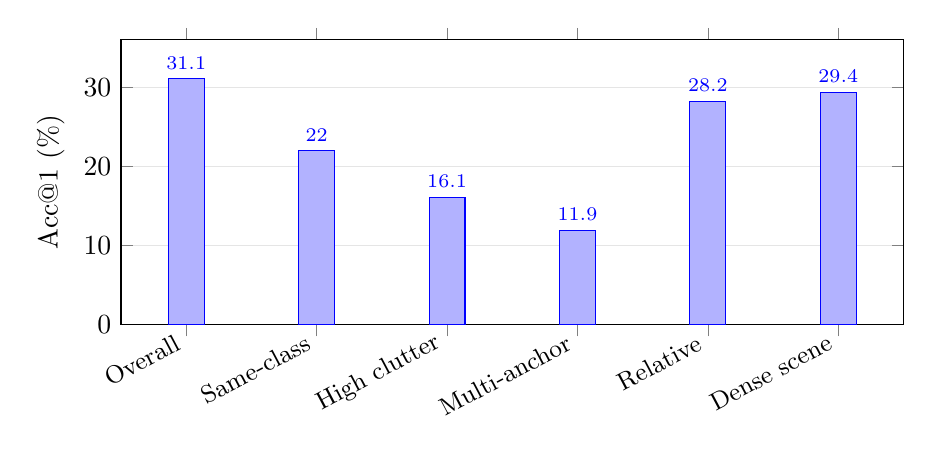
\begin{tikzpicture}
\begin{axis}[
  width=0.95\linewidth,
  height=5.2cm,
  ybar,
  bar width=13pt,
  ymin=0,
  ymax=36,
  ylabel={\acc{} (\%)},
  symbolic x coords={Overall,SameClass,HighClutter,MultiAnchor,Relative,DenseScene},
  xtick=data,
  xticklabels={Overall,Same-class,High clutter,Multi-anchor,Relative,Dense scene},
  x tick label style={rotate=28, anchor=east, font=\small},
  ymajorgrids=true,
  grid style={draw=black!10},
  nodes near coords,
  nodes near coords style={font=\scriptsize, /pgf/number format/fixed, /pgf/number format/precision=1},
  every axis plot/.append style={fill=ragblue!65, draw=ragblue}
]
\addplot coordinates {
  (Overall,31.05)
  (SameClass,21.96)
  (HighClutter,16.07)
  (MultiAnchor,11.90)
  (Relative,28.20)
  (DenseScene,29.39)
};
\end{axis}
\end{tikzpicture}

  \caption{Hard-subset accuracy chart. Same-class clutter, high clutter, and multi-anchor samples are substantially harder than the overall test set.}
  \label{fig:hard-subsets}
\end{figure}

\begin{table}[!htbp]
\centering
\small
\caption{Scene-disjoint hard-subset diagnostics for the reproduced baseline.}
\label{tab:hard-subsets}
\begin{tabular}{lrrrr}
\toprule
Subset & Count & Share & \acc{} & Gap \\
\midrule
Overall & 4,255 & 100.00\% & 31.05\% & -- \\
Same-class clutter, $\geq 3$ & 2,373 & 55.77\% & 21.96\% & -9.09 \\
High clutter, $\geq 5$ & 697 & 16.38\% & 16.07\% & -14.98 \\
Multi-anchor & 168 & 3.95\% & 11.90\% & -19.15 \\
Single-anchor & 320 & 7.52\% & 26.56\% & -4.49 \\
Relative-position & 1,305 & 30.67\% & 28.20\% & -2.85 \\
Dense scene, $\geq 50$ objects & 752 & 17.67\% & 29.39\% & -1.66 \\
\bottomrule
\end{tabular}
\end{table}

Same-class clutter is the most important failure mode by prevalence: it covers 55.77\% of the test set and loses about nine points relative to the overall score. Multi-anchor samples are smaller but more severe, dropping to 11.90\% \acc{}.

\subsection{Anchor Coverage Diagnostics}

Coverage analysis tests whether sparse anchor selection can even expose useful relational evidence. Under a target-centric nearest-neighbor sparse proxy, top-5 selection covers at least one annotated anchor in 67.87\% of geometry-evaluable anchor samples, but covers all annotated anchors in only 54.20\%.

\begin{figure}[!htbp]
  \centering
  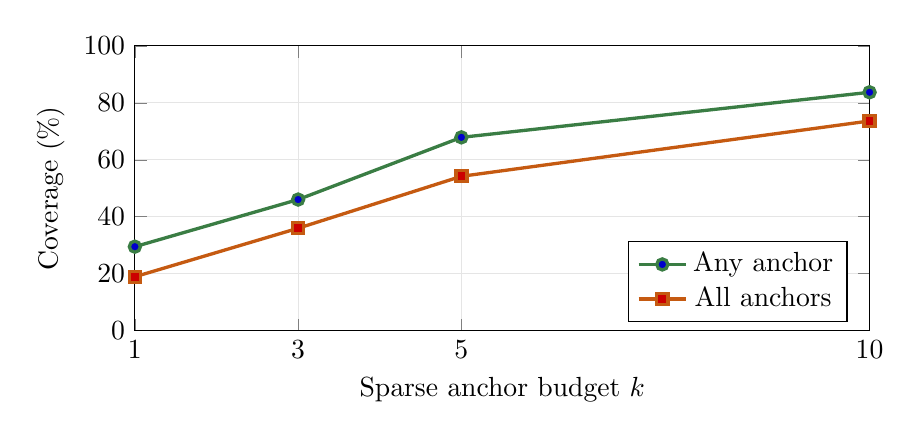
\begin{tikzpicture}
\begin{axis}[
  width=0.9\linewidth,
  height=5.2cm,
  xmin=1,
  xmax=10,
  ymin=0,
  ymax=100,
  xtick={1,3,5,10},
  xlabel={Sparse anchor budget $k$},
  ylabel={Coverage (\%)},
  legend pos=south east,
  ymajorgrids=true,
  xmajorgrids=true,
  grid style={draw=black!10},
  mark options={solid},
]
\addplot+[very thick, color=raggreen, mark=*] coordinates {
  (1,29.50)
  (3,46.04)
  (5,67.87)
  (10,83.69)
};
\addlegendentry{Any anchor}
\addplot+[very thick, color=ragorange, mark=square*] coordinates {
  (1,18.94)
  (3,35.97)
  (5,54.20)
  (10,73.62)
};
\addlegendentry{All anchors}
\end{axis}
\end{tikzpicture}

  \caption{Coverage curve from the coverage diagnostics. The gap between any-anchor and all-anchor coverage shows why multi-anchor expressions are especially fragile under sparse selection.}
  \label{fig:coverage}
\end{figure}

\begin{table}[!htbp]
\centering
\small
\caption{Coverage@k over geometry-evaluable anchor samples.}
\label{tab:coverage}
\begin{tabular}{rrr}
\toprule
$k$ & Any anchor covered & All anchors covered \\
\midrule
1 & 29.50\% & 18.94\% \\
3 & 46.04\% & 35.97\% \\
5 & 67.87\% & 54.20\% \\
10 & 83.69\% & 73.62\% \\
\bottomrule
\end{tabular}
\end{table}

The more direct error-coupled result is that sparse top-5 misses every annotated anchor in 110 of 324 baseline-wrong, anchor-evaluable samples, or 33.95\%. It misses at least one annotated anchor in 157 of 324 such samples, or 48.46\%. Dense all-pair candidate-anchor coverage recovers those anchors at the candidate-set level. This does not prove that a learned reranker will rank correctly, but it establishes that sparse coverage is a genuine bottleneck.

\subsection{Dense Relation Diagnostic Line}

The dense relation line produced one small retained gain and several negative results. Table~\ref{tab:dense} summarizes the outcome. The useful conclusion is not that dense scoring is solved, but that relation evidence is fragile: simple dense reranking can help slightly, while more complex calibration, attention, geometry, and hard-negative variants can amplify noise.

\begin{table}[!htbp]
\centering
\small
\caption{Dense relation diagnostic results under the frozen-logit diagnostic line.}
\label{tab:dense}
\begin{tabular}{lrrrl}
\toprule
Method & Test \acc{} & Test \acctopfive{} & Net & Status \\
\midrule
Clean base & 30.83\% & 91.87\% & -- & Reference \\
Dense-no-cal-v1 & 31.05\% & 92.01\% & +9 & Retained \\
Dense-calibrated-v2 & 30.55\% & 91.80\% & -12 & Frozen \\
Dense-v2-AttPool & 25.24\% & 79.95\% & -238 & Frozen \\
Dense-v3-Geo & 24.32\% & 79.06\% & -277 & Frozen \\
Dense-v4-HardNeg & 24.47\% & 79.41\% & -271 & Frozen \\
\bottomrule
\end{tabular}
\end{table}

\subsection{Controlled Conditioned Architecture Result}

The strongest method evidence is the Phase 4 rerun. The current report uses corrected aggregate summaries derived from the raw three-seed result files. The main comparison is clear: E1 and E3 are about 1.9 points above E0, while E1 and E3 are nearly identical.

\begin{figure}[!htbp]
  \centering
  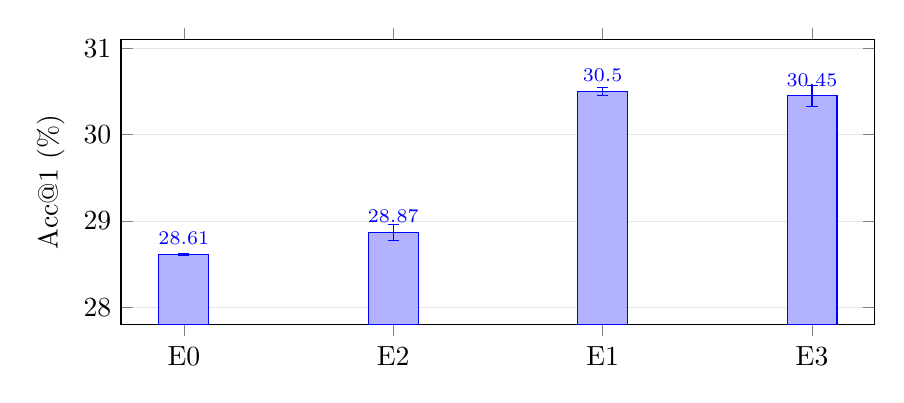
\begin{tikzpicture}
\begin{axis}[
  width=0.92\linewidth,
  height=5.2cm,
  ybar,
  bar width=18pt,
  ymin=27.8,
  ymax=31.1,
  ylabel={\acc{} (\%)},
  symbolic x coords={E0,E2,E1,E3},
  xtick=data,
  ymajorgrids=true,
  grid style={draw=black!10},
  nodes near coords,
  nodes near coords style={font=\scriptsize, /pgf/number format/fixed, /pgf/number format/precision=2},
  error bars/y dir=both,
  error bars/y explicit,
  every axis plot/.append style={draw=ragblue, fill=ragblue!62}
]
\addplot coordinates {
  (E0,28.61) +- (0,0.01)
  (E2,28.87) +- (0,0.09)
  (E1,30.50) +- (0,0.05)
  (E3,30.45) +- (0,0.12)
};
\end{axis}
\end{tikzpicture}

  \caption{Phase 4 ablation chart. Error bars show sample standard deviation across three seeds. The conditioned variants improve over E0, but supervision and no-supervision variants are effectively tied.}
  \label{fig:phase4}
\end{figure}

\begin{table}[!htbp]
\centering
\small
\caption{Controlled Phase 4 rerun. Values are mean $\pm$ sample standard deviation across seeds 42, 123, and 2026.}
\label{tab:phase4}
\begin{tabular}{llrrr}
\toprule
ID & Configuration & Params & \acc{} & \acctopfive{} \\
\midrule
E0 & Dense relation baseline & 398K & $28.61 \pm 0.01$ & $88.13 \pm 0.05$ \\
E2 & Near parameter-matched dense control & 622K & $28.87 \pm 0.09$ & $88.97 \pm 0.05$ \\
E1 & Conditioned + viewpoint supervision & 623K & $30.50 \pm 0.05$ & $91.09 \pm 0.06$ \\
E3 & Conditioned, no viewpoint supervision & 623K & $30.45 \pm 0.12$ & $91.04 \pm 0.05$ \\
\bottomrule
\end{tabular}
\end{table}

The E1--E0 gap is +1.89 points, and E1--E3 is only +0.05 points. This argues against the simple claim that explicit viewpoint supervision drives the gain. The near parameter-matched E2 control has almost the same parameter count as E1 but remains 1.63 points below E1, so the gain is not explained by parameter count alone. However, newer negative controls also matter: the frozen-random and shuffled-viewpoint controls report 30.61\% and 30.53\% \acc{}, respectively, which are essentially tied with E1. The safest interpretation is therefore that the architecture benefits from conditional computation, not that it learns a semantically meaningful viewpoint signal.

\subsection{Pilot Components}

Phase 5 and Phase 6 are implementation checks for additional training paths, not main-claim evidence. The counterfactual objective gives a +0.12 point one-epoch validation gain over its matched baseline, with active counterfactual loss. The random hard-negative control is inconclusive because it never activates under the current embeddings-only data format. The latent-mode pilot gives a small +0.09 point one-epoch signal for $K=4$ over $K=1$, but $K=4$ also uses many more parameters and requires full training before any claim can be made.

\FloatBarrier

\section{Discussion and Limitations}

\paragraph{The main contribution is partly diagnostic.}
The most trustworthy evidence in the repository is the scene-disjoint evaluation and the diagnostic analysis around it. This is appropriate for the course project because it demonstrates a complete empirical workflow: dataset recovery, baseline reproduction, hard-subset analysis, coverage diagnosis, method implementation, ablation, and negative-result reporting.

\paragraph{Viewpoint supervision should not be overclaimed.}
The original idea emphasized viewpoint labels. The current ablations do not support that framing. E1 and E3 have the same architecture, but E3 removes viewpoint supervision and matches E1. The random and shuffled controls further weaken any claim that a learned semantic viewpoint signal is responsible. The report therefore uses the more conservative \method{} framing.

\paragraph{Multi-anchor reasoning remains unsolved.}
Diagnostics show that multi-anchor expressions are difficult, and coverage analysis explains why sparse anchor selection is risky. However, the conditioned scorer does not yet improve multi-anchor accuracy in the controlled ablation. Anchor-chain reasoning remains an important future direction rather than a completed result.

\paragraph{The embeddings-only pipeline limits controls.}
The efficient embedding format stores object embeddings, language features, base logits, and class indices, but not full per-object metadata such as class names and 3D centers. This makes some geometry-aware controls impossible, especially random hard negatives based on spatial proximity. A metadata-preserving extraction path is needed for stronger counterfactual ablations.

\paragraph{Some evidence remains pilot-level.}
The Phase 5 counterfactual and Phase 6 latent-mode runs are one-epoch pilots on the validation split. They are useful implementation checks, but they should not be treated as final claims. Full 80-epoch latent-mode training with multiple seeds is planned but not yet complete in the current repository state.

\section{Conclusion}

This project investigates relation-aware 3D visual grounding under a verified scene-disjoint evaluation protocol. The strongest current findings are that the reproduced baseline fails systematically on same-class clutter and multi-anchor cases, sparse anchor selection misses a substantial fraction of useful anchor evidence, and conditional relation computation improves over a controlled dense relation baseline.

The final method claim is intentionally conservative. The project does not show state-of-the-art performance, does not solve multi-anchor grounding, and does not validate explicit viewpoint supervision. It does show a credible research progression from diagnosis to method testing: \method{} is a useful architectural direction, while full latent-mode training, metadata-preserving controls, and stronger multi-anchor reasoning remain future work.


\FloatBarrier
\begingroup
\small
\setlength{\bibsep}{0pt plus 0.3ex}
\bibliographystyle{plainnat}
\bibliography{references}
\endgroup

\end{document}
